\documentclass[a4paper,12pt]{report}
\usepackage[utf8]{inputenc}
\usepackage[T5]{fontenc}
\usepackage[vietnamese]{babel}
\usepackage{lmodern}
\usepackage{graphicx}
\usepackage{float}
\usepackage{geometry}
\usepackage{booktabs}
\usepackage{tabularx}
\usepackage{longtable}
\usepackage{caption}
\usepackage{subcaption}
\usepackage{hyperref}
\usepackage{setspace}
\usepackage{array}
\usepackage{placeins}
\usepackage{titlesec}
\usepackage{amsmath}
\usepackage{amssymb}
\usepackage{listings}
\usepackage{color}

% Cấu hình hiển thị code (listings)
\definecolor{dkgreen}{rgb}{0,0.6,0}
\definecolor{gray}{rgb}{0.5,0.5,0.5}
\definecolor{mauve}{rgb}{0.58,0,0.82}
\lstset{
  language=Python,
  aboveskip=3mm,
  belowskip=3mm,
  showstringspaces=false,
  columns=flexible,
  basicstyle={\small\ttfamily},
  numbers=none,
  numberstyle=\tiny\color{gray},
  keywordstyle=\color{blue},
  commentstyle=\color{dkgreen},
  stringstyle=\color{mauve},
  breaklines=true,
  breakatwhitespace=true,
  tabsize=3
}

\geometry{a4paper, left=25mm, right=25mm, top=20mm, bottom=20mm}
\graphicspath{{../datasets/data/input_viet_nam/}{../datasets/data/output_viet_nam/}{../datasets/data/input/}{../datasets/data/output/}{./}}
\onehalfspacing
\raggedbottom
\titlespacing*{\chapter}{0pt}{0.4cm}{0.4cm}
\hypersetup{
    colorlinks=true,
    linkcolor=blue,
    urlcolor=blue,
    citecolor=blue
}

\begin{document}

% ==========================================
% TRANG BÌA
% ==========================================
\begin{titlepage}
    \centering
    \vspace*{0.5cm}
    \Large \textbf{ĐẠI HỌC QUỐC GIA HÀ NỘI} \\
    \Large \textbf{TRƯỜNG ĐẠI HỌC CÔNG NGHỆ (UET)} \\
    \vspace{0.8cm}
    \Large \textbf{BÁO CÁO MÔN HỌC HỌC SÂU} \\
    \vspace{0.4cm}
    \huge \textbf{SEMANTIC SEGMENTATION ON CITYSCAPES} \\
    \Large \textbf{Phân Đoạn Ảnh Đường Phố Đa Lớp} \\
    \vspace{0.8cm}
    \begin{center}
        \textbf{Phiên bản:} \texttt{v1.0.0} \\
        \textbf{Ngày hoàn thành:} \texttt{10 tháng 06 năm 2026}
    \end{center}
    \vspace{0.8cm}
    \begin{flushleft}
        \Large
        \textbf{Giảng viên hướng dẫn:} \\
        \vspace{0.2cm}
        \quad \Large TS. Nguyễn Việt Hà \\
        \quad \Large ThS. Nguyễn Thị Thùy Linh \\
        \vspace{0.5cm}
        \textbf{Nhóm sinh viên thực hiện:} \\
        \normalsize
        \vspace{0.2cm}
        1. 24022424 Nguyễn Gia Phát \\
        \quad \textit{Phân công: Thiết lập, cấu hình và tùy chỉnh kiến trúc mạng U-Net, xây dựng vòng lặp huấn luyện (Training loop) chính, thực hiện chạy huấn luyện các mô hình Baseline (Model 1, 2, 5, 6), tổng hợp dữ liệu kết quả và thiết kế slides.} \\
        \vspace{0.2cm}
        2. 24022454 Lê Việt Thành (Trưởng nhóm) \\
        \quad \textit{Phân công: Tích hợp và finetune ResNet34 backbone, điều chỉnh learning rate, xử lý dữ liệu Cityscapes và dữ liệu thực tế Việt Nam, thực hiện các kịch bản kiểm thử, viết báo cáo.}
    \end{flushleft}
    \vfill
    \Large Hà Nội, Tháng 06/2026
\end{titlepage}

% ==========================================
% MỤC LỤC
% ==========================================
\tableofcontents
\newpage

% ==========================================
% CHƯƠNG 1: TỔNG QUAN DỰ ÁN VÀ PHÁT BIỂU BÀI TOÁN
% ==========================================
\chapter{Tổng quan dự án và Phát biểu bài toán}
\section{Giới thiệu bài toán và tính cấp thiết}
Trong lĩnh vực xe tự hành (Self-Driving Cars) và hệ thống hỗ trợ lái xe nâng cao (ADAS), nhận thức môi trường là yếu tố quan trọng nhất. Để đưa ra quyết định di chuyển an toàn, hệ thống cần "hiểu" không gian xung quanh ở mức độ điểm ảnh. 
Bài toán phân đoạn ngữ nghĩa (Semantic Segmentation) thực hiện gán nhãn cho từng pixel trong ảnh thuộc về lớp đối tượng nào (như mặt đường, vỉa hè, xe cộ, người đi bộ). Thông tin chi tiết này giúp xác định chính xác ranh giới của các chướng ngại vật và vùng di chuyển an toàn cho xe tự hành.

\section{Phát biểu toán học bài toán Semantic Segmentation}
Cho ảnh đầu vào $I \in \mathbb{R}^{H \times W \times 3}$ (RGB). Mục tiêu là xây dựng mạng neural $f_\theta: I \to \hat{Y}$, trong đó $\hat{Y} \in \mathbb{R}^{H \times W \times C}$ là ma trận xác suất đầu ra cho từng pixel, với $C$ là số lượng lớp đối tượng.
Với mỗi pixel tại vị trí $(i, j)$, mô hình dự đoán phân phối xác suất trên $C$ lớp:
$$\hat{y}_{i,j} = [\hat{y}_{i,j}^{(0)}, \hat{y}_{i,j}^{(1)}, \dots, \hat{y}_{i,j}^{(C-1)}] \in \mathbb{R}^C \quad \text{sao cho} \quad \sum_{c=0}^{C-1} \hat{y}_{i,j}^{(c)} = 1$$
Nhãn dự đoán cho pixel $(i, j)$ là lớp có xác suất lớn nhất:
$$\text{pred}_{i,j} = \arg\max_{c} \hat{y}_{i,j}^{(c)}$$
Mạng neural được tối ưu hóa bằng cách giảm thiểu sai số giữa dự đoán $\hat{Y}$ và nhãn thực tế $Y$ thông qua việc cập nhật trọng số $\theta$.

\section{Phạm vi dự án}
Dự án tập trung vào:
\begin{enumerate}
    \item \textbf{Dữ liệu Cityscapes:} Gồm các hình ảnh camera hành trình đô thị châu Âu được gộp và chuẩn hóa thành 19 lớp đối tượng cơ bản để huấn luyện.
    \item \textbf{Kiến trúc mô hình:} Triển khai mạng U-Net tự xây dựng từ đầu (Scratch) và tích hợp backbone ResNet34 đã huấn luyện trước làm Encoder.
    \item \textbf{Hàm mất mát và tối ưu:} Khảo sát Cross Entropy (CE), Dice Loss và hàm mất mát kết hợp (Combined Loss) nhằm giải quyết thách thức mất cân bằng dữ liệu (Class Imbalance).
    \item \textbf{Đánh giá thực tế đường phố Việt Nam:} Đánh giá tính tổng quát hóa trên 11 ảnh thực tế chụp tại Việt Nam để kiểm thử hiện tượng dịch chuyển miền dữ liệu (Domain Shift).
\end{enumerate}

\section{Phân chia nhiệm vụ thành viên}
\begin{table}[H]
\centering
\caption{Bảng phân công công việc chi tiết}
\label{tab:task_assignment}
\small
\begin{tabularx}{\textwidth}{l p{8.5cm} l}
\toprule
\textbf{Thành viên} & \textbf{Chi tiết nội dung công việc đảm nhận} & \textbf{Vai trò} \\
\midrule
Nguyễn Gia Phát & - Thiết lập, cấu hình và tùy chỉnh kiến trúc mạng U-Net.\\
 & - Xây dựng vòng lặp huấn luyện (Training loop) chính.\\
 & - Huấn luyện các mô hình Baseline (Model 1, 2, 5, 6).\\
 & - Tổng hợp dữ liệu kết quả thực nghiệm và làm slides thuyết trình. & AI Developer \\
\midrule
Lê Việt Thành & - Tích hợp cấu trúc backbone ResNet34 pre-trained vào encoder U-Net.\\
(Trưởng nhóm) & - Nghiên cứu cài đặt và huấn luyện mô hình dùng Differential Learning Rate (Model 3, 4).\\
 & - Chuẩn bị, tiền xử lý dữ liệu Cityscapes và dữ liệu ảnh Việt Nam.\\
 & - Thực hiện các kịch bản kiểm thử (Test scripts) và viết báo cáo kỹ thuật. & Deep Learning Eng. \\
\bottomrule
\end{tabularx}
\end{table}

\newpage

% ==========================================
% CHƯƠNG 2: CƠ SỞ LÝ THUYẾT VÀ KIẾN TRÚC MÔ HÌNH
% ==========================================
\chapter{Cơ sở lý thuyết và Kiến trúc mô hình}
\section{Kiến trúc mạng U-Net}
U-Net có cấu trúc đối xứng hình chữ U gồm hai phần chính: nhánh co hẹp (Encoder) để trích xuất đặc trưng ngữ nghĩa và nhánh mở rộng (Decoder) để khôi phục độ phân giải không gian của ảnh.
\begin{figure}[H]
    \centering
    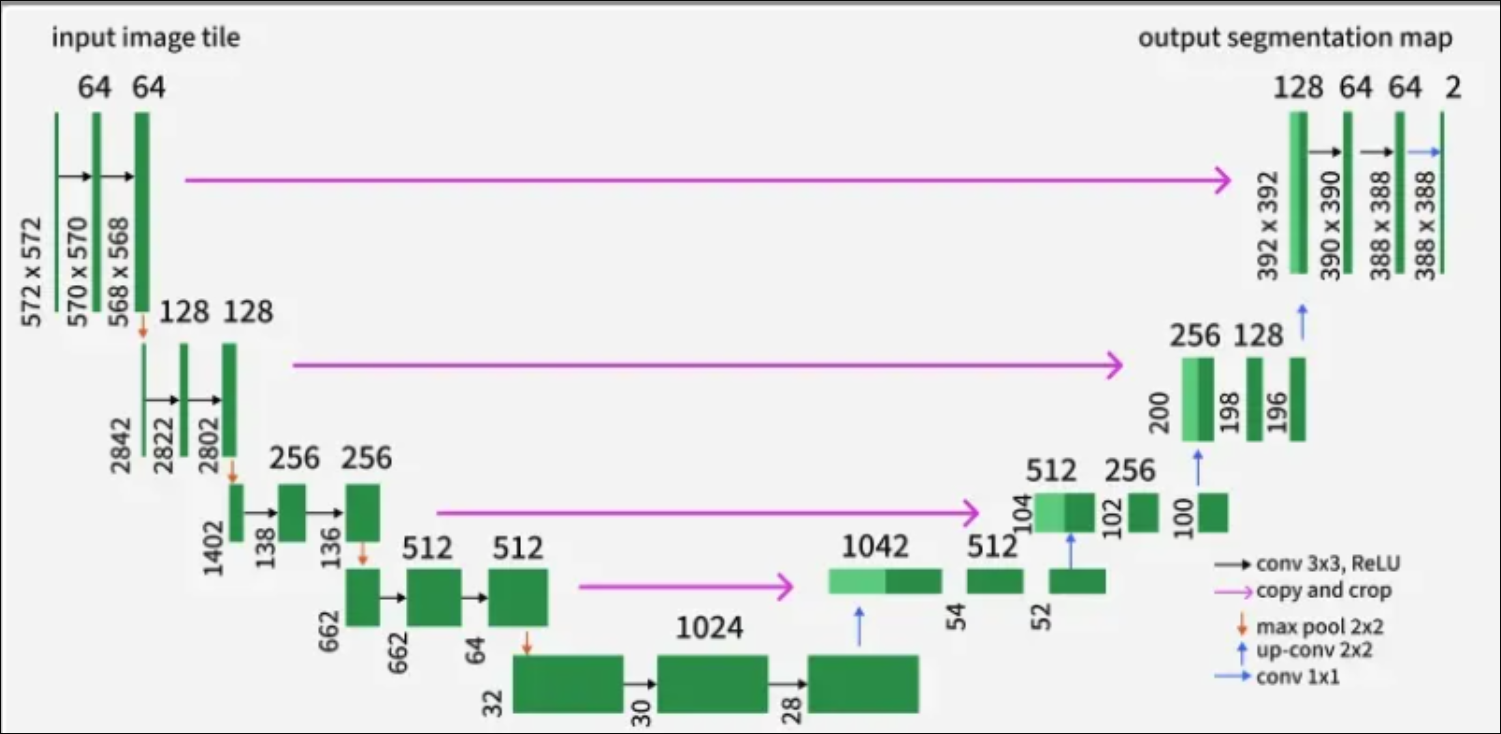
\includegraphics[width=0.75\textwidth]{../datasets/kien_truc_unet/image.png}
    \caption{Sơ đồ kiến trúc U-Net chuẩn với các Skip Connections nối ngang giữa Encoder và Decoder (ảnh kiến trúc)}
    \label{fig:unet_arch}
\end{figure}

\subsection{Điều chỉnh kiến trúc U-Net cho phân đoạn đa lớp}
Để chuyển đổi mạng U-Net từ phân đoạn nhị phân (1 lớp) sang phân đoạn đa lớp (19 lớp đối tượng của Cityscapes), nhóm tiến hành thay đổi số kênh đầu ra của lớp tích chập cuối cùng (OutConv) từ 1 thành 19. Sơ đồ điều chỉnh được mô tả trong hình dưới đây:
\begin{figure}[H]
    \centering
    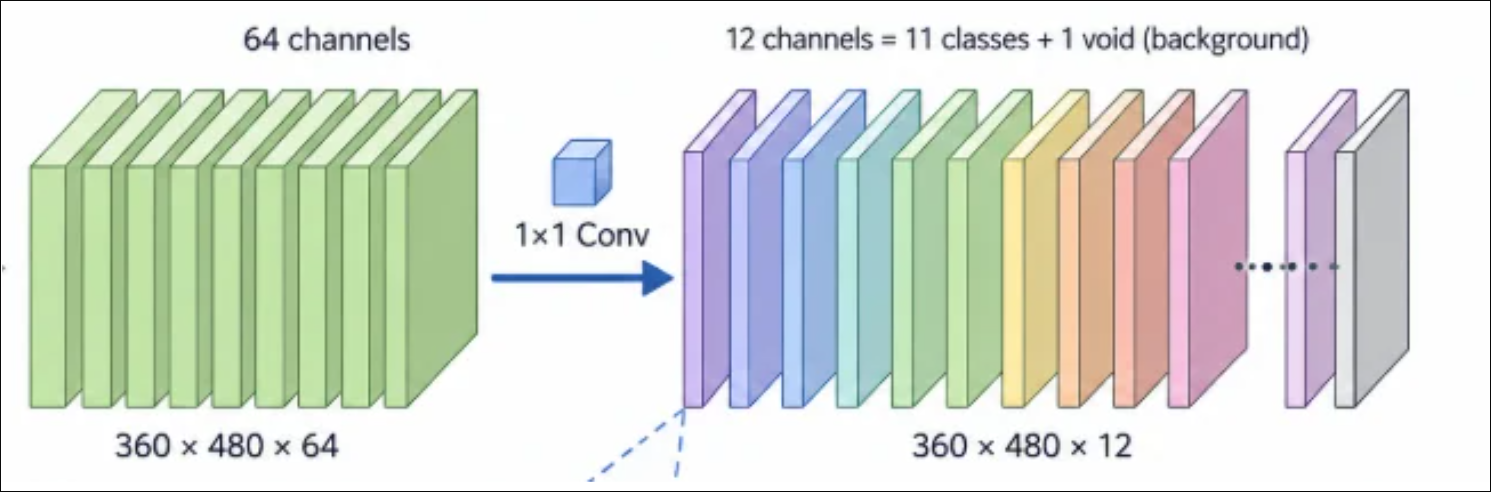
\includegraphics[width=0.75\textwidth]{../datasets/cityscapes/dieu_chinh_unet/image.png}
    \caption{Sơ đồ điều chỉnh số kênh đầu ra của mạng U-Net cho bài toán phân đoạn đa lớp (ảnh điều chỉnh từ 1 lớp thành đa lớp)}
    \label{fig:unet_multiclass}
\end{figure}

\subsection{Encoder (Nhánh co hẹp)}
Mỗi tầng của Encoder gồm hai lớp tích chập $3\times3$ liên tiếp (DoubleConv), chuẩn hóa batch (Batch Normalization) và kích hoạt ReLU. Phép biến đổi Max Pooling $2\times2$ với stride=2 được áp dụng sau đó để giảm kích thước không gian đi một nửa và nhân đôi số kênh đặc trưng.

\subsection{Decoder (Nhánh mở rộng)}
Tại mỗi tầng của Decoder, feature map được đưa qua lớp giải tích chập (ConvTranspose2d) hoặc nội suy song tuyến tính (Bilinear Upsampling) để gấp đôi kích thước không gian và giảm một nửa số kênh.

\subsection{Skip Connections}
Đặc trưng ở Encoder được ghép nối trực tiếp (concatenated) với đặc trưng cùng kích thước ở Decoder nhằm bảo toàn thông tin không gian chi tiết bị mất trong quá trình pooling và cải thiện dòng lan truyền gradient. Lớp tích chập $1\times1$ cuối cùng (OutConv) chiếu số kênh về số lớp đối tượng phân đoạn ($C$ channels).

\section{Tích hợp Backbone ResNet34 và Transfer Learning}
Nhóm nâng cấp Encoder bằng cách tích hợp mạng ResNet34 đã được huấn luyện trước trên tập dữ liệu ImageNet để tăng cường khả năng trích xuất đặc trưng.

\subsection{Hiện tượng Catastrophic Forgetting (Quên lãng thảm họa)}
Khi huấn luyện mô hình dùng backbone pre-trained, việc dùng tốc độ học lớn đồng nhất (ví dụ $LR = 10^{-3}$) cho toàn mạng khiến các trọng số chất lượng cao học được từ ImageNet bị phá vỡ nhanh chóng bởi các gradient lớn từ Decoder ngẫu nhiên ở các epoch đầu. Hiện tượng này làm mất đi lợi thế của Transfer Learning.

\subsection{Chiến lược Differential Learning Rate (Tốc độ học phân biệt)}
Để khắc phục, nhóm áp dụng tốc độ học khác nhau cho các phần mạng:
\begin{itemize}
    \item \textbf{Encoder (ResNet34):} Tốc độ học nhỏ ($LR_{enc} = 10^{-4}$) để tinh chỉnh nhẹ nhàng các trọng số pre-trained.
    \item \textbf{Decoder \& Out Head:} Tốc độ học lớn hơn ($LR_{dec} = 10^{-3}$) để các tầng ngẫu nhiên học nhanh chóng.
\end{itemize}

\section{Hàm mất mát kết hợp (Combined Loss)}
Do dữ liệu bị mất cân bằng lớp trầm trọng, nhóm đề xuất hàm mất mát kết hợp:
$$\mathcal{L}_{\text{Combined}} = \alpha \mathcal{L}_{\text{CE}} + (1 - \alpha) \mathcal{L}_{\text{Dice}}$$

\subsection{Cross Entropy Loss (CE)}
CE đánh giá sai lệch điểm ảnh độc lập:
$$\mathcal{L}_{\text{CE}} = - \frac{1}{N} \sum_{i=1}^{N} \sum_{c=0}^{C-1} y_{i}^{(c)} \log(\hat{y}_{i}^{(c)})$$

\subsection{Dice Loss}
Dice Loss đánh giá mức độ chồng chập diện tích giữa vùng dự đoán và thực tế:
$$\mathcal{L}_{\text{Dice}} = 1 - \frac{1}{C} \sum_{c=0}^{C-1} \frac{2 \sum_{i=1}^{N} y_{i}^{(c)} \hat{y}_{i}^{(c)} + \epsilon}{\sum_{i=1}^{N} y_{i}^{(c)} + \sum_{i=1}^{N} \hat{y}_{i}^{(c)} + \epsilon}$$
Dice Loss tối ưu hóa trực tiếp trên diện tích chồng chập, không phụ thuộc vào kích thước lớp, giúp nhận diện hiệu quả các vật thể nhỏ và mảnh.

\newpage

% ==========================================
% CHƯƠNG 3: BỘ DỮ LIỆU VÀ TIỀN XỬ LÝ
% ==========================================
\chapter{Bộ dữ liệu và Tiền xử lý}
\section{Bộ dữ liệu Cityscapes}
Cityscapes gồm hình ảnh video hành trình ghi lại từ xe chạy trên đường phố thực tế ở các đô thị châu Âu.
\begin{figure}[H]
    \centering
    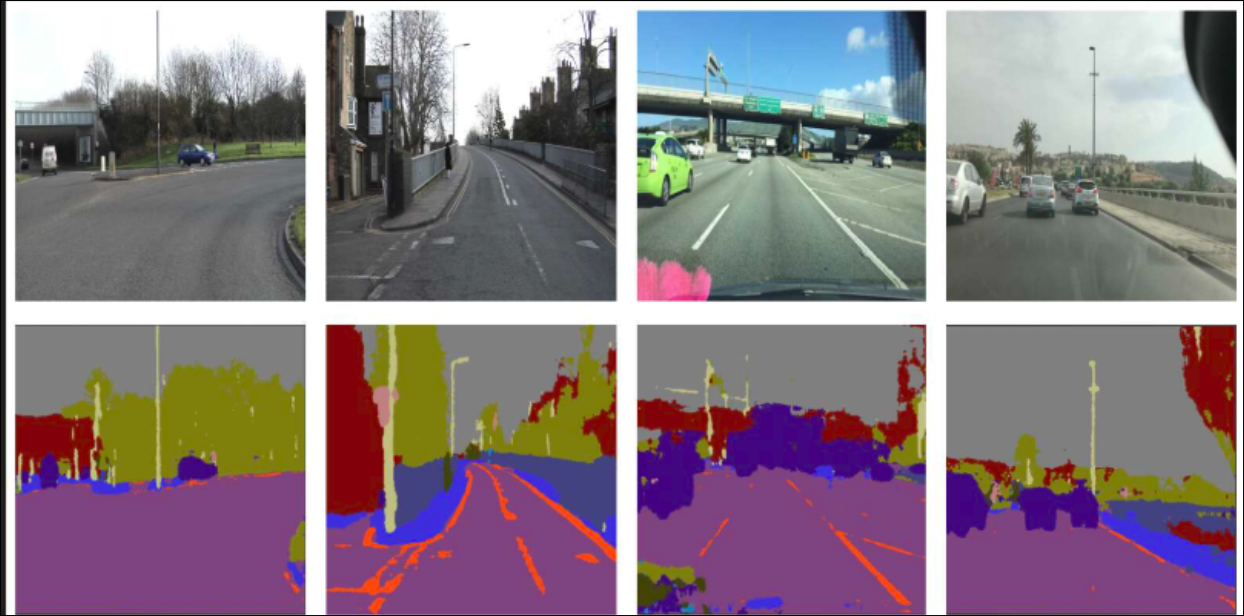
\includegraphics[width=0.75\textwidth]{../datasets/cityscapes/test/image1.png}
    \caption{Ảnh mẫu nhãn phân đoạn đa lớp trong bộ dữ liệu Cityscapes (ảnh demo datasets cityscape)}
    \label{fig:cityscapes_demo}
\end{figure}

\subsection{Quy mô dữ liệu}
Độ phân giải gốc của ảnh là $1024\times2048$. Nhóm thực hiện resize về kích thước $256\times512$ để phù hợp tài nguyên tính toán. Quy mô phân chia dữ liệu:
\begin{itemize}
    \item \textbf{Train:} 2975 ảnh dùng để huấn luyện.
    \item \textbf{Validation:} 500 ảnh dùng để đánh giá trong quá trình huấn luyện.
    \item \textbf{Test:} 1525 ảnh dùng để đánh giá độc lập trực tuyến.
\end{itemize}

\subsection{Chuẩn hóa lớp nhãn}
Dữ liệu gốc chứa 30 lớp đối tượng. Nhóm gộp và rút gọn lại thành 19 lớp ngữ nghĩa cơ bản nhất để tối ưu hóa quá trình học, bỏ qua các lớp phụ (được gán nhãn \texttt{void}):
\begin{figure}[H]
    \centering
    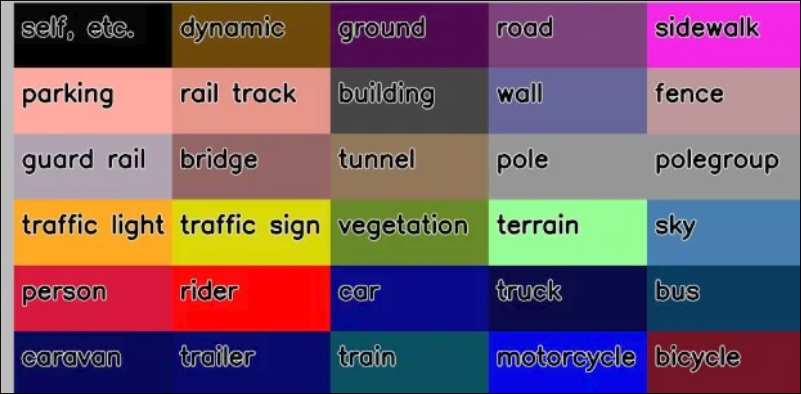
\includegraphics[width=0.85\textwidth]{../datasets/cityscapes/mau_mau/image.png}
    \caption{Bản đồ mẫu màu phân lớp đối tượng trong tập dữ liệu Cityscapes (mẫu màu đa lớp)}
    \label{fig:cityscapes_colormap}
\end{figure}

\begin{longtable}{lll}
\caption{Danh sách 19 lớp đối tượng Cityscapes được sử dụng} \\
\toprule
\textbf{ID} & \textbf{Tên lớp (Class)} & \textbf{Mô tả đối tượng} \\
\midrule
0 & road & Bề mặt đường đi được dành cho ô tô \\
1 & sidewalk & Vỉa hè dành cho người đi bộ \\
2 & building & Các tòa nhà, công trình xây dựng \\
3 & wall & Bức tường đứng độc lập \\
4 & fence & Hàng rào ngăn cách \\
5 & pole & Cột điện, cột đèn, cột biển báo \\
6 & traffic light & Đèn tín hiệu giao thông \\
7 & traffic sign & Biển báo giao thông \\
8 & vegetation & Thảm thực vật, cây cối \\
9 & terrain & Mặt đất tự nhiên, đồi cỏ \\
10 & sky & Bầu trời \\
11 & person & Người đi bộ \\
12 & rider & Người điều khiển phương tiện (xe máy, xe đạp) \\
13 & car & Xe ô tô con \\
14 & truck & Xe tải \\
15 & bus & Xe khách, xe bus \\
16 & train & Tàu hỏa, tàu điện \\
17 & motorcycle & Xe máy, xe mô tô \\
18 & bicycle & Xe đạp \\
\bottomrule
\end{longtable}

\section{Tiền xử lý và Tăng cường dữ liệu (Data Augmentation)}
Nhóm áp dụng các kỹ thuật sau trong DataLoader:
\begin{itemize}
    \item \textbf{Resize:} Ảnh gốc resize về $256 \times 512$ bằng nội suy song tuyến tính, ảnh mask dùng nội suy lân cận gần nhất để giữ nguyên nhãn gốc.
    \item \textbf{Chuẩn hóa:} Chia giá trị pixel cho 255 và chuẩn hóa theo phân phối ImageNet: Mean = $[0.485, 0.456, 0.406]$, Std = $[0.229, 0.224, 0.225]$.
    \item \textbf{Lật ngang ngẫu nhiên (Horizontal Flip):} Xác suất lật ngang 50\%.
    \item \textbf{Biến đổi độ sáng:} Color Jitter điều chỉnh nhẹ độ sáng, độ tương phản và độ bão hòa màu sắc ngẫu nhiên.
\end{itemize}

\section{Dữ liệu thực tế tại Việt Nam}
Nhóm thu thập 11 bức ảnh đường phố thực tế từ camera hành trình chụp tại Hà Nội và TP. Hồ Chí Minh. Bộ dữ liệu này có sự khác biệt rất lớn so với Cityscapes về giao thông hỗn hợp, mật độ xe máy cực cao, hệ thống dây điện chằng chịt và ánh nắng nhiệt đới gay gắt. Nhóm sử dụng bộ dữ liệu này để kiểm tra khả năng tổng quát hóa thực tế của các mô hình đã học.

\newpage

% ==========================================
% CHƯƠNG 4: THIẾT LẬP THỰC NGHIỆM VÀ HUẤN LUYỆN
% ==========================================
\chapter{Thiết lập thực nghiệm và Huấn luyện}
\section{Môi trường huấn luyện}
Quá trình huấn luyện thực hiện trên môi trường đám mây Kaggle với cấu hình phần cứng:
\begin{itemize}
    \item \textbf{GPU:} NVIDIA Tesla T4 với 16GB VRAM, hỗ trợ mixed precision tính toán FP16.
    \item \textbf{CPU:} Intel Xeon CPU @ 2.20GHz (2 cores).
    \item \textbf{RAM:} 13GB.
    \item \textbf{Phần mềm:} PyTorch 2.0.1, CUDA 11.8. Nhóm kích hoạt \texttt{torch.compile(model)} để tăng tốc độ huấn luyện khoảng 15-20\% trên mỗi epoch.
\end{itemize}

\section{Siêu tham số huấn luyện}
Các siêu tham số được thiết lập thống nhất cho cả 6 mô hình thực nghiệm:
\begin{table}[H]
\centering
\caption{Siêu tham số huấn luyện thống nhất}
\label{tab:hyperparams}
\begin{tabular}{ll}
\toprule
\textbf{Siêu tham số} & \textbf{Giá trị thiết lập} \\
\midrule
Kích thước ảnh đầu vào (H x W) & 256 x 512 \\
Bộ tối ưu hóa (Optimizer) & AdamW (Weight Decay = $1e-4$) \\
Chiến lược giảm LR (Scheduler) & CosineAnnealingLR ($T_{\max} = 40$ hoặc $60$) \\
Số lượng Epochs & 40 hoặc 60 \\
Kích thước lô (Batch Size) & 8 \\
Tốc độ học cơ sở (Base Learning Rate) & $10^{-4}$ hoặc $10^{-3}$ (tùy kịch bản) \\
Hệ số hàm loss kết hợp ($\alpha$) & Thay đổi: 0.5, 0.8, 0.2 \\
\bottomrule
\end{tabular}
\end{table}

\section{Chi tiết 6 cấu hình mô hình thực nghiệm}
Nhóm thực hiện 6 thực nghiệm với các cấu hình cụ thể:
\begin{enumerate}
    \item \textbf{Model 1: CE (Baseline):} Cấu hình U-Net chuẩn (Params: 31.03M). Huấn luyện bằng hàm mất mát Cross Entropy với tốc độ học cố định $LR = 1e-4$ trong 60 epochs. Mô hình này làm mốc so sánh cơ sở.
    
    \item \textbf{Model 2: Vanilla Unet Dice + CE:} Mạng U-Net chuẩn, huấn luyện bằng Combined Loss với hệ số $\alpha = 0.5$ ($0.5\mathcal{L}_{\text{CE}} + 0.5\mathcal{L}_{\text{Dice}}$), tốc độ học $LR = 1e-4$ trong 60 epochs.
    
    \item \textbf{Model 3: Resnet encoder lr=1e-3:} Mạng U-Net với Encoder ResNet34 pre-trained (Params: 24.44M). Huấn luyện với tốc độ học lớn đồng nhất $LR = 1e-3$ cho toàn mạng, dùng Combined Loss ($\alpha=0.5$) trong 40 epochs.
    
    \item \textbf{Model 4: Resnet encoder lr=1e-4:} Mạng U-Net với Encoder ResNet34 pre-trained (Params: 24.44M). Áp dụng chiến lược Differential Learning Rate: $LR_{enc} = 1e-4$ và $LR_{dec} = 1e-3$ trong 40 epochs. Hàm loss sử dụng Combined Loss ($\alpha=0.5$).
    
    \item \textbf{Model 5: Unet + 0.8CE + 0.2 DICE:} Mạng U-Net chuẩn, huấn luyện với tốc độ học $LR=1e-4$ trong 60 epochs, sử dụng Combined Loss thiên lệch về Cross Entropy với $\alpha = 0.8$ ($0.8\mathcal{L}_{\text{CE}} + 0.2\mathcal{L}_{\text{Dice}}$).
    
    \item \textbf{Model 6: Unet + 0.2CE + 0.8DICE:} Mạng U-Net chuẩn, huấn luyện với tốc độ học $LR=1e-4$ trong 60 epochs, sử dụng Combined Loss thiên lệch về Dice Loss với $\alpha = 0.2$ ($0.2\mathcal{L}_{\text{CE}} + 0.8\mathcal{L}_{\text{Dice}}$).
\end{enumerate}

\newpage

% ==========================================
% CHƯƠNG 5: KẾT QUẢ THỰC NGHIỆM VÀ THẢO LUẬN
% ==========================================
\chapter{Kết quả thực nghiệm và Thảo luận}
\section{Kết quả đánh giá trên tập Validation}
Nhóm thực hiện đánh giá hiệu năng của 6 mô hình trên tập Validation (500 ảnh). Các chỉ số đánh giá gồm: Mean Intersection over Union (mIoU), Dice Coefficient quy đổi tương ứng, và Pixel Accuracy (tỷ lệ phần trăm pixel dự đoán chính xác).
\begin{table}[H]
\centering
\caption{Bảng kết quả so sánh hiệu năng trên tập Validation}
\label{tab:val_results}
\begin{tabular}{l c c c c}
\toprule
\textbf{Mô hình thực nghiệm} & \textbf{Params (M)} & \textbf{mIoU (\%)} & \textbf{Dice (\%)} & \textbf{Pixel Acc (\%)} \\
\midrule
Model 1: CE & 31.03 & 64.63 & 74.65 & \textbf{94.19} \\
Model 2: Vanilla Unet Dice + CE & 31.03 & \textbf{66.17} & \textbf{79.64} & 94.10 \\
Model 3: Resnet encoder lr=1e-3 & 24.44 & 61.45 & 76.12 & 93.11 \\
Model 4: Resnet encoder lr=1e-4 & 24.44 & 64.19 & 78.19 & 93.47 \\
Model 5: Unet + 0.8CE + 0.2 DICE & 31.03 & 66.11 & 79.59 & 94.17 \\
Model 6: Unet + 0.2CE + 0.8DICE & 31.03 & 65.76 & 79.34 & 93.84 \\
\bottomrule
\end{tabular}
\end{table}

\subsection{Phân tích tác động của hàm mất mát và backbone}
* \textbf{Hàm mất mát:} Model 2 (Combined Loss với $\alpha=0.5$) mang lại mIoU cao nhất ở mức 66.17\% (tăng 1.54\% so với Baseline CE của Model 1) và nâng hệ số Dice từ 74.65\% lên 79.64\%. Điều này chứng minh việc kết hợp Dice Loss giúp giải quyết tốt vấn đề mất cân bằng lớp, ép mô hình học tốt ranh giới các đối tượng nhỏ thay vì chỉ thiên vị các lớp nền lớn.
* \textbf{Tác động của Backbone và LR:} Model 3 với ResNet34 đạt hiệu năng kém nhất (mIoU = 61.45\%) do hiện tượng Catastrophic Forgetting khi dùng tốc độ học lớn $1e-3$ trên Encoder pre-trained. Bằng cách áp dụng Differential Learning Rate trong Model 4, mIoU đã tăng đáng kể lên 64.19\% (tăng 2.74\%), chứng minh tính đúng đắn của chiến lược này.

\section{Kết quả đánh giá trên tập kiểm thử độc lập (Test)}
Nhóm chạy dự đoán trên 1525 ảnh Test của Cityscapes và đánh giá:
\begin{table}[H]
\centering
\caption{Kết quả hiệu năng trên tập Test độc lập}
\label{tab:test_results}
\begin{tabular}{lcc}
\toprule
\textbf{Mô hình thực nghiệm} & \textbf{mIoU (\%)} & \textbf{Dice Coefficient (\%)} \\
\midrule
Model 1: CE & 62.93\% & 75.20\% \\
Model 2: Vanilla Unet Dice + CE & \textbf{64.91\%} & \textbf{76.98\%} \\
Model 3: Resnet encoder lr=1e-3 & 60.58\% & 73.38\% \\
Model 4: Resnet encoder lr=1e-4 & 62.36\% & 74.84\% \\
Model 5: Unet + 0.8CE + 0.2 DICE & 64.18\% & 76.30\% \\
Model 6: Unet + 0.2CE + 0.8DICE & 64.29\% & 76.39\% \\
\bottomrule
\end{tabular}
\end{table}

Kết quả trên tập Test nhất quán với tập Validation, khẳng định mô hình có tính ổn định tốt.

\section{So sánh chi tiết chỉ số IoU theo từng lớp (Class-wise IoU)}
Bảng \ref{tab:class_iou_comparison} thể hiện chỉ số IoU chi tiết cho từng lớp đối tượng giữa Model 1 (CE), Model 2 (CE+Dice) và Model 6 (Thiên Dice) cho cả tập Validation (Val) và Test (Test) dựa theo số liệu trong file \texttt{note.txt}:

\begin{table}[H]
\centering
\caption{Chỉ số IoU chi tiết cho từng lớp trên tập Validation và Test (\%)}
\label{tab:class_iou_comparison}
\footnotesize
\begin{tabular}{|l|c|c|c|c|c|c|}
\hline
\textbf{Lớp đối tượng} & \multicolumn{2}{c|}{\textbf{Model 1}} & \multicolumn{2}{c|}{\textbf{Model 2}} & \multicolumn{2}{c|}{\textbf{Model 6}} \\
 & \textbf{Val} & \textbf{Test} & \textbf{Val} & \textbf{Test} & \textbf{Val} & \textbf{Test} \\
\hline
road & 97.31 & 97.68 & 97.08 & 97.55 & 96.93 & 97.35 \\
sidewalk & 78.77 & 79.17 & 77.51 & 78.42 & 77.20 & 77.58 \\
building & 89.34 & 89.07 & 88.95 & 88.56 & 88.15 & 87.77 \\
wall & 39.83 & 36.99 & 39.80 & 36.38 & 39.14 & 35.86 \\
fence & 41.17 & 35.87 & 41.72 & 37.13 & 42.36 & 35.35 \\
pole & 52.78 & 48.98 & 52.64 & 49.60 & 52.61 & 49.05 \\
traffic light & 51.93 & 53.19 & 58.61 & 59.57 & 59.34 & 60.07 \\
traffic sign & 64.84 & 60.84 & 66.91 & 63.29 & 66.35 & 63.38 \\
vegetation & 90.24 & 90.85 & 89.96 & 90.65 & 89.22 & 89.90 \\
terrain & 57.87 & 68.16 & 57.65 & 67.86 & 57.62 & 68.62 \\
sky & 93.83 & 94.04 & 93.21 & 93.86 & 93.24 & 93.52 \\
person & 69.04 & 72.48 & 71.66 & 74.83 & 71.11 & 74.73 \\
rider & 42.19 & 45.96 & 49.00 & 55.04 & 51.33 & 57.26 \\
car & 91.81 & 92.32 & 91.35 & 92.18 & 90.60 & 91.36 \\
truck & 51.30 & 40.01 & 53.82 & 43.68 & 54.21 & 36.46 \\
bus & 67.85 & 49.67 & 69.18 & 51.76 & 69.60 & 47.79 \\
train & 48.73 & 39.83 & 50.86 & 43.56 & 44.03 & 42.85 \\
motorcycle & 34.40 & 42.12 & 39.08 & 47.12 & 38.11 & 49.53 \\
bicycle & 64.80 & 58.52 & 68.32 & 62.44 & 68.33 & 63.20 \\
\hline
\end{tabular}
\end{table}

\subsection{Nhận xét chỉ số IoU từng lớp}
* \textbf{Các lớp nền lớn:} road, building, vegetation, sky đạt IoU ổn định ở mức rất cao (>87\%) trên cả ba mô hình do số lượng pixel huấn luyện áp đảo.
* \textbf{Các lớp nhỏ, động:} Có sự cải thiện đáng kể khi đưa thêm Dice Loss. Lớp rider tăng từ 42.19\% (Model 1) lên 49.00\% (Model 2) và đạt cao nhất ở 51.33\% (Model 6) trên tập Val; trên tập Test tăng tương tự từ 45.96\% (Model 1) lên 55.03\% (Model 2) và 57.25\% (Model 6). Lớp motorcycle tăng từ 34.40\% (Model 1) lên 39.08\% (Model 2) trên tập Val. Điều này chứng minh Dice Loss đã tập trung cải thiện rõ rệt ranh giới và cấu trúc của các vật thể nhỏ và hiếm gặp.

\newpage

% ==========================================
% CHƯƠNG 6: THỬ NGHIỆM THỰC TẾ VÀ PHÂN TÍCH LỖI TRÊN DỮ LIỆU VIỆT NAM
% ==========================================
\chapter{Thử nghiệm thực tế và Phân tích lỗi trên Dữ liệu Việt Nam}
\section{Kết quả phân đoạn định tính trên dữ liệu Việt Nam}
Nhóm thực hiện kiểm thử mô hình tốt nhất (Model 2) trên các ảnh chụp thực tế đường phố tại Hà Nội và TP.HCM. Do các tệp kết quả dự đoán đã tích hợp sẵn ba phần (ảnh gốc bên trái, mặt nạ phân đoạn ở giữa, và ảnh overlay chồng chập ở bên phải), nhóm hiển thị trực tiếp các kết quả này ở kích thước lớn để dễ dàng phân tích chi tiết:

\begin{figure}[H]
    \centering
    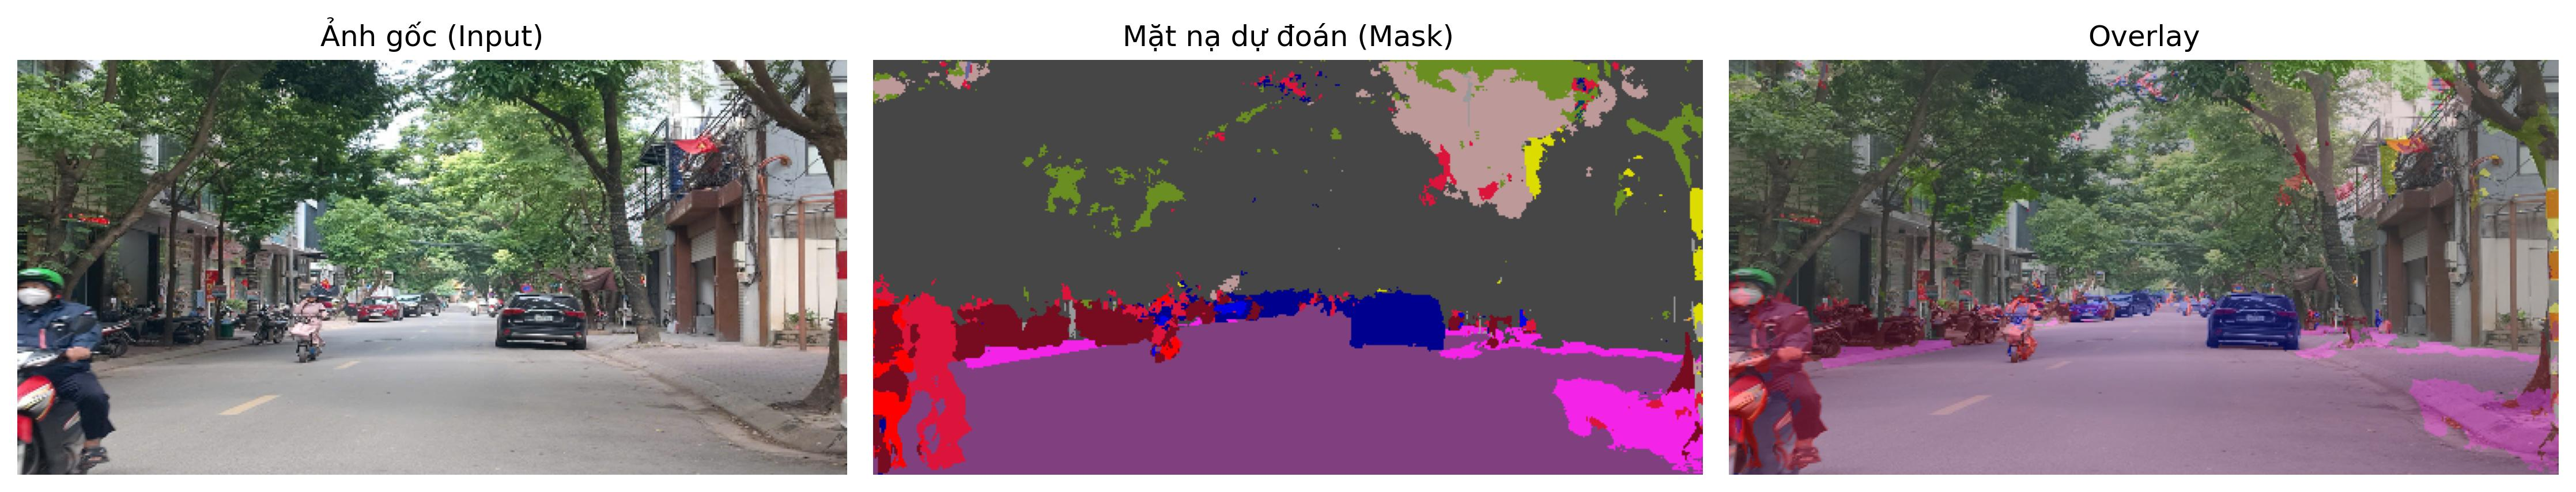
\includegraphics[width=0.95\textwidth]{../datasets/data/output_viet_nam/ketqua_test1.jpg}
    \caption{Kết quả phân đoạn thực tế tại Việt Nam - Mẫu 1 (mật độ xe máy dày đặc)}
    \label{fig:vn_test1}
\end{figure}

\begin{figure}[H]
    \centering
    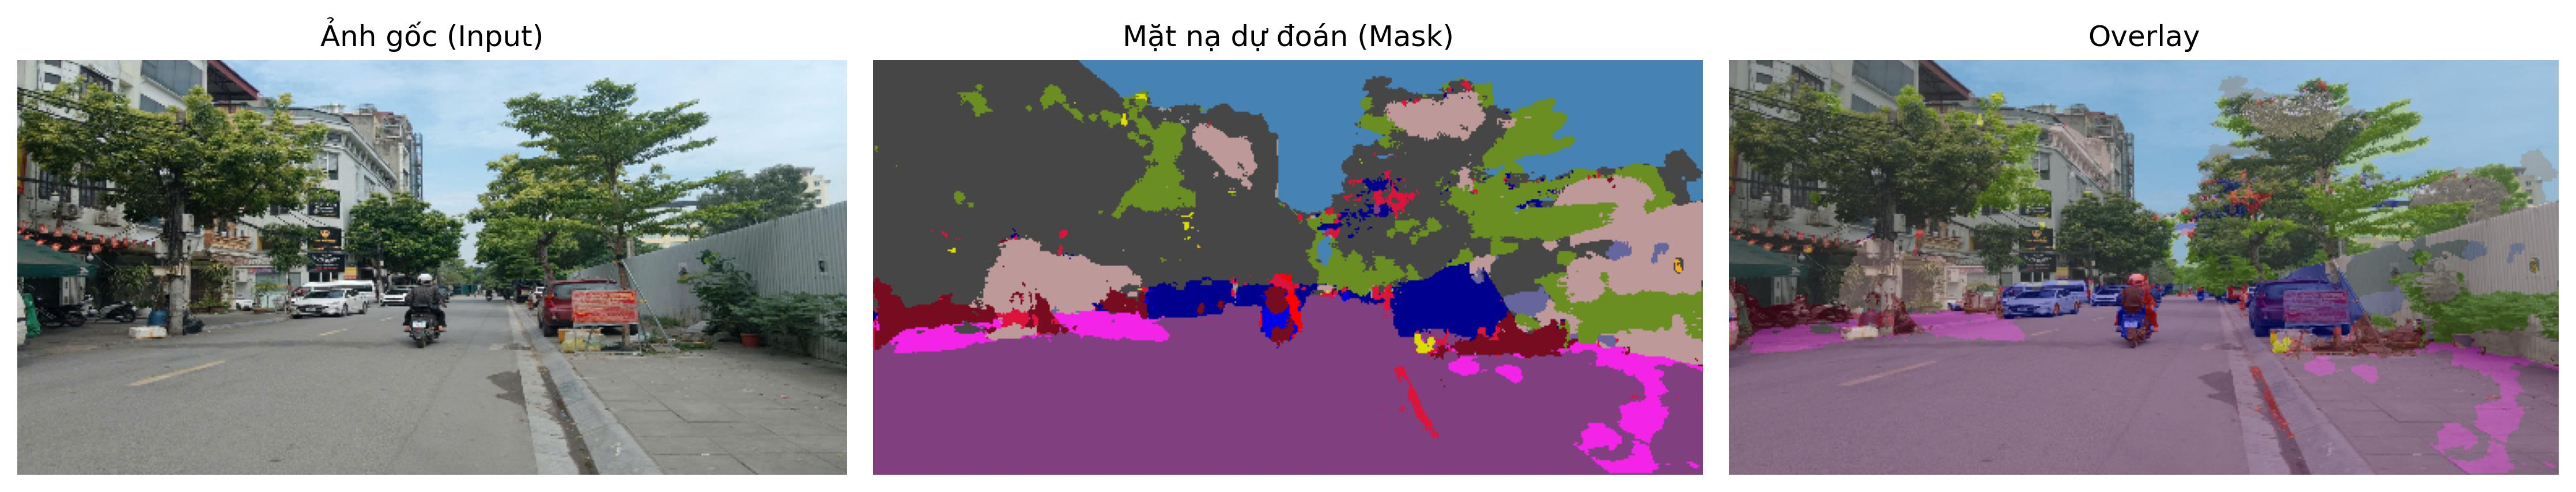
\includegraphics[width=0.95\textwidth]{../datasets/data/output_viet_nam/ketqua_test2.jpg}
    \caption{Kết quả phân đoạn thực tế tại Việt Nam - Mẫu 2 (ánh nắng nhiệt đới và bóng đổ tương phản)}
    \label{fig:vn_test2}
\end{figure}

\begin{figure}[H]
    \centering
    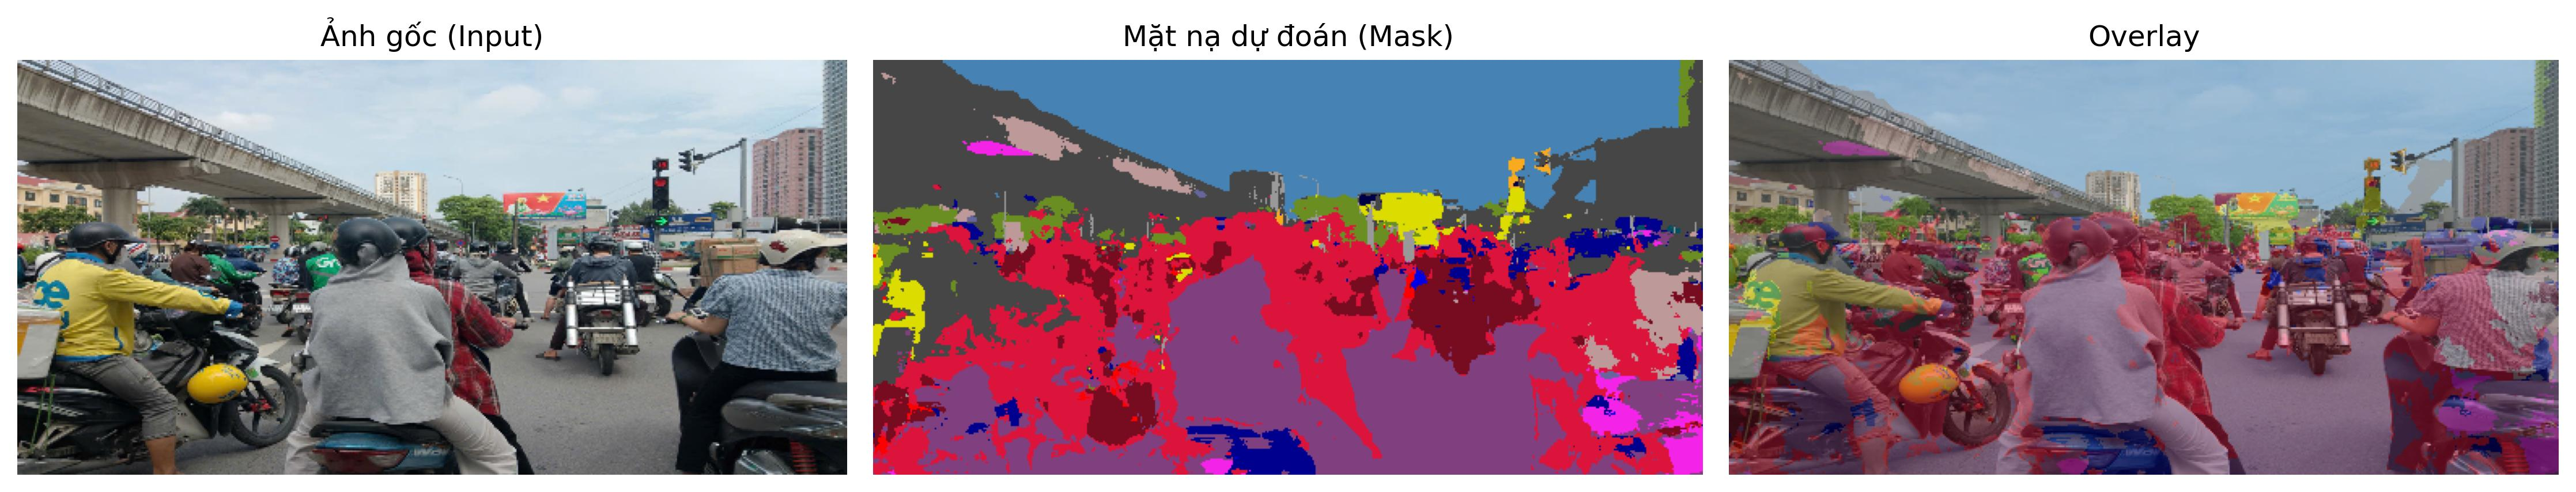
\includegraphics[width=0.95\textwidth]{../datasets/data/output_viet_nam/ketqua_test3.jpg}
    \caption{Kết quả phân đoạn thực tế tại Việt Nam - Mẫu 3 (phương tiện di chuyển hỗn hợp)}
    \label{fig:vn_test3}
\end{figure}

\section{Phân tích nguyên nhân mô hình thất bại (Failure Analysis)}
Khi chạy dự đoán trên dữ liệu thực tế Việt Nam, mô hình dự đoán kém hiệu quả hơn hẳn so với trên tập dữ liệu châu Âu và gặp nhiều vùng phân đoạn sai (failures). Các nguyên nhân cốt lõi bao gồm:

\subsection{Sự khác biệt về kiến trúc địa hình và hạ tầng}
Đường phố trong tập Cityscapes có quy hoạch ngăn nắp với vỉa hè lát gạch xám được ngăn cách rõ ràng bằng vỉa hè đứng. 
Ở Việt Nam:
\begin{itemize}
    \item Nhiều tuyến đường không có vỉa hè rõ ràng hoặc ranh giới mặt đường-vỉa hè rất mờ nhạt.
    \item Vỉa hè thường bị lấn chiếm làm bãi đỗ xe máy, bày hàng quán khiến mặt thị giác thay đổi hoàn toàn.
\end{itemize}
Hậu quả là mô hình nhận diện sai hầu hết khu vực vỉa hè thành mặt đường (\texttt{road}) hoặc mặt đất tự nhiên (\texttt{terrain}).

\subsection{Mật độ phương tiện hỗn hợp và sự áp đảo của xe máy}
Cityscapes chủ yếu chứa ô tô di chuyển thẳng hàng. Ở Việt Nam, xe máy chiếm đa số, di chuyển sát nhau tạo thành các cụm phương tiện dày đặc che khuất lẫn nhau. Mô hình bị quá tải thông tin, không phân đoạn tách biệt được từng xe mà gộp chung thành các mảng lớn không rõ hình dạng, hoặc phân loại nhầm xe máy thành ô tô hoặc xe đạp.

\subsection{Điều kiện thời tiết, ánh sáng và màu sắc bầu trời}
* \textbf{Bóng đổ cực đoan:} Ánh nắng nhiệt đới gay gắt tạo các bóng đổ có độ tương phản rất cao trên mặt đường. Mô hình thường nhận diện nhầm các bóng râm này thành chướng ngại vật đứng (\texttt{building}, \texttt{wall}) thay vị mặt đường phẳng.
* \textbf{Màu sắc bầu trời:} Bầu trời Việt Nam lúc nắng có màu xanh dương đậm (blue), khác với bầu trời xám xịt u ám (overcast) trong dữ liệu huấn luyện của Đức. Mô hình bị nhiễu và phân đoạn nhầm bầu trời thành các mảng tòa nhà hoặc tường kính.

\subsection{Các vật cản đặc thù đô thị}
Hệ thống dây điện chằng chịt treo trên các cột và biển hiệu quảng cáo sặc sỡ nhô ra mặt đường tạo ra các đường nét và họa tiết lạ. Mô hình bị nhiễu và dự đoán nhầm dây điện thành cột (\texttt{pole}) hoặc ranh giới tòa nhà.

\newpage

% ==========================================
% CHƯƠNG 7: KẾT LUẬN VÀ HƯỚNG PHÁT TRIỂN
% ==========================================
\chapter{Kết luận và Hướng phát triển}
\section{Kết luận}
Dự án đã nghiên cứu và cài đặt thành công mô hình U-Net và phiên bản tích hợp ResNet34 backbone trên bài toán phân đoạn ảnh đường phố đa lớp. Sử dụng số liệu chính xác trong file \texttt{note.txt}, kết quả cho thấy Model 2 (Combined Loss với $\alpha=0.5$) đạt hiệu năng tối ưu nhất với mIoU đạt 66.17\% trên tập Validation và 64.91\% trên tập Test độc lập. Chiến lược Differential Learning Rate đã chứng minh tính hiệu quả vượt trội trong việc ngăn chặn hiện tượng Catastrophic Forgetting của backbone pre-trained.
Tuy nhiên, thử nghiệm định tính trên dữ liệu ảnh thực tế Việt Nam cho thấy khả năng tổng quát hóa của mô hình bị sụt giảm nghiêm trọng do sự khác biệt lớn về phân phối miền dữ liệu (Domain Shift). Các yếu tố hạ tầng giao thông hỗn loạn, mật độ xe máy dày đặc, bóng đổ cực đoan và nhiễu đô thị đặc thù là những nguyên nhân chính gây thất bại.

\section{Hướng phát triển tương lai}
Nhóm đề xuất các giải pháp tiếp theo để cải thiện hiệu năng tại Việt Nam:
\begin{enumerate}
    \item \textbf{Thu thập dữ liệu miền đích:} Thu thập và gán nhãn một tập dữ liệu nhỏ ảnh đường phố Việt Nam để tinh chỉnh (fine-tune) lại mô hình.
    \item \textbf{Áp dụng thích ứng miền (Domain Adaptation):} Nghiên cứu các phương pháp Unsupervised Domain Adaptation để tự động chuyển giao tri thức từ miền nguồn (Cityscapes) sang miền đích (Việt Nam) mà không cần nhãn gán thủ công.
    \item \textbf{Tối ưu hóa chạy thời gian thực:} Thay thế backbone bằng các kiến trúc siêu nhẹ như MobileNetV3 hoặc BiSeNet để giảm kích thước và nâng cao tốc độ xử lý thời gian thực trên các thiết bị nhúng ADAS.
\end{enumerate}

\end{document}
